\documentclass[12pt]{article}

\usepackage[russian]{babel}
\usepackage{amssymb}

\usepackage[export]{adjustbox}

\title{Алгоритм Natasha-2}
\begin{document}

\maketitle
 
\section{Постановка задачи}

$$ \min_{x \in \mathbb{R}} f(x) = \frac{1}{n}\sum_{i=1}^n f_i(x)  = \mathbb{E}_i [f_i(x)], $$

где ${f_i}$ --- в общем случае невыпуклые функции.

Будет построен онлайн-алгоритм (т.е. не зависящий от $n$), находящий локальный минимум с заданной точностью.

\section{Необходимые предположения}

\begin{itemize}

	\item f имеет ограниченную дисперсию, откуда $\mathbb{E}_i \left[ \Vert \nabla f_i(x) - \nabla f(x) \Vert \right]$
	\item $L$-Липшицевость градиента: $\Vert \nabla f(x) - \nabla f(y) \Vert \leq L \cdot \Vert x -y \Vert$

	%\item все собственные значения $\nabla^2 f(x)$ лежат на отрезке $[-\sigma, L]$
	\item $L_2$-Липшицевость гессиана: $\Vert \nabla^2 f(x) - \nabla^2 f(y) \Vert \leq L_2 \cdot \Vert x -y \Vert$
	
\end{itemize}


\section{Определения }

\begin{itemize}

	\item Локальный минимум с $(\varepsilon, \delta)$-точностью -  точка $x$, такая что $\Vert \nabla f(x) \Vert < \varepsilon$ и  $\nabla^2 f(x) \succeq -\delta \mathbf{I}$ (все собственные значения гессиана больше $-\delta$).

	\item $\sigma$-невыпуклая функция - функция, такая что минимальное собственное значение её гессиана превосходит $-\sigma$
\end{itemize}



\section{Описание алгоритма}

Главная идея - использование гессиана для избегания седловых точек.

\subsection{Carmon: Сведение к поиску стационарных точек}


%Близость $y$ к седловой точке $x$, такая что $\Vert x-y \Vert \leq \delta$ влечёт существование такого $v$, что $v^T \nabla^2 f(y) v \leq -\frac{\delta}{2} $.

На каждой итерации в точке $y_k$ сравниваем минимальное собственное значение $\lambda_{min}(\nabla^2f(y_k))$ и $- \delta$.
\begin{itemize}
	\item Если $\exists v : v^T \nabla^2f(y_k) v \leq -\frac{\delta}{2} $, то пытаемся отдалиться от седла: $y_{k+1} = y_k \pm \frac{\delta}{L_2}v$ ($+$ или $-$ выбираем случайно)
		
	\item Иначе берём $F^k(x) = f(x) + L(\max\{ 0, \Vert x - y_k \Vert - \frac{\delta}{L_2} \})^2$, которая явялется $5L$-Липшицевой по градиенту и $3\delta$-невыпуклой; ищем для неё точку $\widehat{x} : \Vert \nabla F^k(\widehat{x}) \Vert \leq \varepsilon$ и переходим туда: $y_{k+1} = \widehat{x}$. Как видно, $F^k$ штрафует за выход из <<безопасной зоны>> $\{x : \Vert x - y_k \Vert \leq \frac{\delta}{L_2} \}$
	
\end{itemize}

\subsection{Natasha 1.5: Поиск стационарных точек для $\sigma$-невыпуклых функций}

Каждая эпоха делится на $p = \Theta((\frac{\sigma}{\varepsilon L})^{\frac{2}{3}})$ суб-эпох со стартовым вектором $\widehat{x}$.\\

Затем, при подсчёте градиентов, вместо $f(x)$ фактически используется $f(x) + \sigma \Vert x - \widehat{x} \Vert^2$, что должно стабилизировать алгоритм, немного замедляя его.
Вместе с этим, используется пересчёт градиента из алгоритма SVRG

\newpage
 
Псевдокод:

\adjustbox{center}{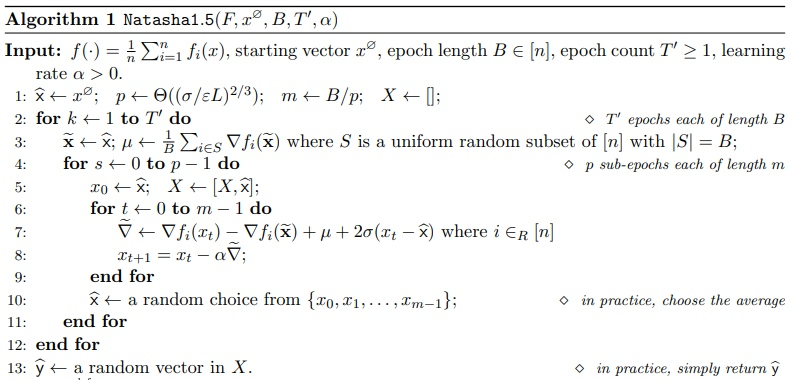
\includegraphics[scale=0.5]{Natasha-1dot5.jpg}}

\subsection{Oja: Быстрый поиск максимального собственного значения}

%\section{Алгоритмы}

%\subsection{Natasha 1.5}

%\subsection{Oja's algorithm}

%\subsection{Natasha 2}


 
  
\end{document}